{\color{gray}\hrule}
\begin{center}
\section{Appendices}
%\textbf{Small description}
\bigskip
\end{center}
{\color{gray}\hrule}
\begin{multicols}{2}
\subsection{Code Structure}
\begin{verbatim}
    exec
     |   - main // Executable
    include
     |   - AmericanOption.cpp
     |   - AmericanOption.h
     |   - AsianOption.cpp
     |   - AsianOption.h
     |   - EuropeanOption.cpp
     |   - EuropeanOption.h
     |   - MonteCarlo.h
     |   - Option.h
    lib  {external libraries}
     |   - boost/
     |   - eigen/
    src
     |   - main.cpp
\end{verbatim}
\subsection{Definitions}
\begin{itemize}
    \item \textbf{Discretization Errors:} Errors that may arise when continuous mathematical features like time are approximated using discrete steps in numerical simulations.
    \item \textbf{Continuation Value Approximation:} The continuation value in option pricing refers to the expected value of holding an option and not exercising it immediately, under a risk-neutral measure.
    \item \textbf{Regression Order:} The regression order refers to the degree of the polynomial used to approximate the continuation value of the option. A higher regression order allows for a more flexible and accurate fit of the continuation value function to the simulated asset prices. 
    \item \textbf{Geometric Brownian Motion:} A stochastic process used to model the price of the underlying asset in the Black-Scholes framework.
    \item \textbf{Volatility:} A measure of the uncertainty or variability in the price of the underlying asset.
    \item \textbf{Multithreading:} A parallel programming technique that divides computational tasks among multiple CPU cores for faster performance.
    \item \textbf{Memoization:} A computational optimization technique that caches previously calculated results for reuse to avoid redundant computations.
\end{itemize}

\subsection{Graphs}
\subsubsection{LSM \& BBSR Comparison}
The graph (Figure 4) illustrates the tradeoff between computational effort and accuracy in the Longstaff-Schwartz Monte Carlo (LSM) method. While the BBSR method produces stable and accurate results across all parameters, the LSM method converges to the correct price only when the sample size (\(N\)) and the number of time steps (\(M\)) are sufficiently large.
\end{multicols}
\begin{figure}[H]
    \centering
    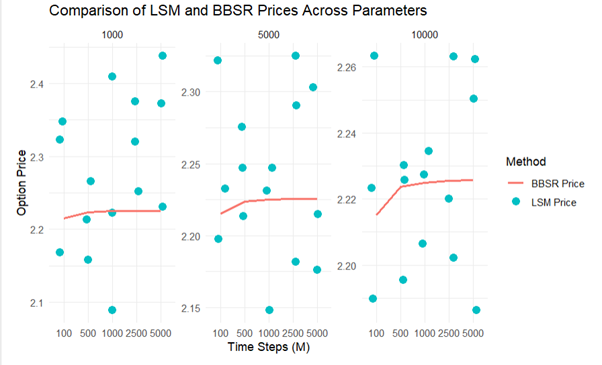
\includegraphics[width=1\linewidth]{Picture6.png}
    \caption{LSM \& BBSR Comparison}
    \label{fig:enter-label}
\end{figure}

\href{https://gitlab.engr.illinois.edu/mbhang2/ie522_final_project.git}{GitLab Code Repository}